\documentclass{article}
\usepackage{graphicx}
\usepackage{listings}
\usepackage{color}
\usepackage[utf8]{inputenc}

\title{Sperimentazione sui tempi di CPU del metodo PageRank\\
	Corso di LSMC, a.a. 2017-2018}
\author{Davide Gori\\
	550282}


\definecolor{backcolour}{rgb}{0.95,0.95,0.92}
\definecolor{gray}{rgb}{0.5,0.5,0.5}
\lstset{basicstyle=\ttfamily\small,
	columns=fullflexible,
	numbers=left,
	numberstyle=\tiny\ttfamily\color{gray},
	backgroundcolor=\color{backcolour},
	tabsize=4,
	language=Octave
}


\begin{document}
	\maketitle
	
	\section{Obiettivi e descrizione della sperimentazione}
	Vogliamo valutare come i tempi di cpu impiegati dal metodo di PageRank crescono al crescere della dimensione $n$ della matrice di adiacenza. In particolare calcoleremo il tempo medio di esecuzione di un'iterazione dell'algoritmo al variare di $n$ e di $\gamma$.\\
	Per questo realizzeremo due sperimentazioni


	\section{Prima sperimentazione}
	In questo esercizio è stato necessario abbassare i valori di dimensione della matrice di adiacenza a causa della poca potenza e memoria del calcolatore. Di seguito il procedimento eseguito:\\
	\begin{itemize}
		\item Modifichiamo la funzione {\tt PageRank} in {\tt PageRank2}, che restituisce un vettore contenente rispettivamente il ranking, il tempo totale impiegano nelle iterazioni e
		il numero di iterazioni.
		\item per ogni $n=100, 1000, 10000, 100000, 1000000$ generiamo tre matrici sparse (col comando {\tt sprand}) con un numero di elementi non nulli pari a 0.1n, n, 10n.
		\item Invochiamo il comando {\tt PageRank2} e prendiamo il quoziente tra tempo e numero di passi ad ogni chiamata.
	\end{itemize}
	
	\section{Lo script}
	Questa è la funzione usata:
	
	\lstinputlisting{PageRank2.m}
	
	Questo è lo script che realizza la sperimentazione:
	
	\lstinputlisting{s_es2.m}
	
	\section{Risultati}
	
	La tabella seguente riporta i valori in output:
	
	\begin{center}
		\begin{tabular}{c|c|c|c|c}
			$n$ & $el$ & $t$ & $it$ & $ratio$   \\ \hline
			100 & n & 0.0033152 & 40 & 8.2880e-05 \\
			100 & 10n & 0.0026560 & 25 & 1.0624e-04 \\
			100 & 100n & 8.0705e-04 & 2 & 4.0352e-04 \\
			1000 & n & 0.024854 & 174 & 1.4284e-04 \\
			1000 & 10n & 0.0072720 & 25 & 2.9088e-04 \\
			1000 & 100n & 0.023525 & 14 & 0.0016804 \\
			10000 & n & 0.040196 & 54 & 7.4437e-04 \\
			10000 & 10n & 0.056684& 26 & 0.0021802 \\
			10000 & 100n & 0.24388 & 14 & 0.017420 \\
			100000 & n & 20.442 & 179 & 0.11420 \\
			100000 & 10n & 14.392 & 26 & 0.55354 \\
			100000 & 100n & 107.16 & 14 & 7.6546 \\
		\end{tabular}
	\end{center}
	Dove con $el$ si intende il numero di elementi non nulli della matrice, con $t$ il tempo di esecuzione della funzione {\tt PageRank2} e con $ratio$ il rapporto tempo su numero di iterazioni.\\
	Possiamo notare che per il caso $n=100$ non ha senso la densità $100n$, infatti questo significa che la matrice è completamente piena di $1$: non è un caso reale.\\
	Notiamo che all'aumentare della densità diminuisce il numero di passi impiegati dall'algoritmo per raggiungere una certa precisione, ma questo non impedisce al tempo di esecuzione di aumentare: infatti come possiamo notare dal caso $n=10000$ (che è sicuramente il più rappresentativo dell'intera sperimentazione) il tempo impiegato mediamente per ogni singolo passo nel caso $el=100n$ è circa $7.5$ secondi.

	
	\section{Seconda sperimentazione}
	Vogliamo ora studiare come cambia il numero di iterazioni al variare del parametro $\gamma$ (Google consiglia $0.85$).
	Fissiamo la dimensione della matrice di adiacenza a $10000$ e prendiamo un vettore di personalizzazione tale che $v(i)=1$ per ogni $1 \leq i\leq n$. Facciamo variare $\gamma$ e registriamo i tempi di esecuzione dell'algoritmo {\tt PageRank}. Ripetiamo la procedura con tre matrici di adiacenza con numero di elementi rispettivamente $n$, $10n$ e $100n$.\\
	\begin{itemize}
		\item Usiamo la funzione {\tt PageRank2} usata nella precedente sperimentazione, per misurare i tempi.
		\item Per ogni $\gamma=0.5:0.01:0.99$ memorizziamo il numero di iterazioni effettuate dall' algoritmo {\tt PageRank2} con i parametri descritti sopra e matrice di adiacenza di densità $n$.
		\item ripetiamo il punto precedente anche per le altre due densità.
		\item Disegnamo i tre grafici che hanno in ascissa i valori di $\gamma$ e ordinata il numero di iterazioni effettuate.
	\end{itemize}
	
	\section{Lo script}
	
	Questo e\'e lo script che realizza la sperimentazione:
	
	\lstinputlisting{s_es3o.m}
	
	Dove la funzione {\tt PageRank2} è la stessa usata per la prima esperienza.
	
	\section{Risultati}
	
	Riportiamo il grafico in output:
	
	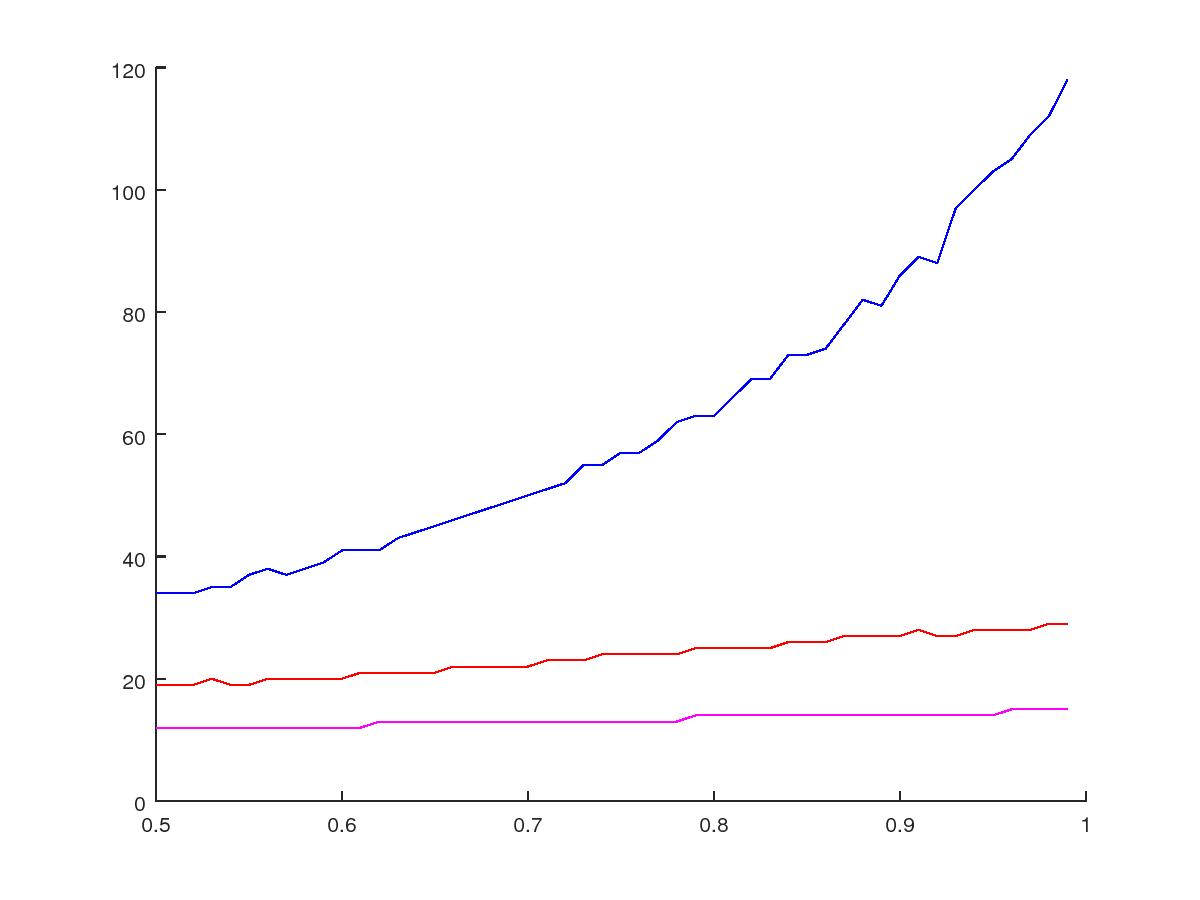
\includegraphics[width=\textwidth]{grafico_es3o.jpeg}
	Dove i grafici blu, rosso e magenta sono relativi alle matrici di adiacenza con un numero di elementi non nulli pari a $n$, $10n$, $100n$.\\
	Si nota subito che più la matrice è sparsa e maggiore è il numero di iterazioni effettuate (in accordo con i risultati dell'esperimento precedente).\\
	Le tre curve sono "grossomodo" crescenti, questo vuol dire che più $\gamma$ è alto (e quindi si ha un'influenza del vettore di personalizzazione minore) più è necessario un maggior numero di iterazioni per ottenere una buona approssimazione.\\
	Guardando invece la derivata delle tre curve si può evincere che questa è più piccola più la densità della matrice di adiacenza è grossa. Sembra inoltre che a densità molto basse la derivata della funzione cresca velocemente e quindi la derivata seconda sia positiva.\\
	Queste osservazioni derivano esclusivamente da una mera osservazione dei dati nel grafico.
\end{document}